\documentclass[12pt]{article}
\usepackage[utf8]{inputenc}

%%% I added a few packages. This next one allows you to set the margins.
\usepackage[top=.5in,bottom=1in,right=.75in,left=.75in]{geometry}
\usepackage{multicol}
%\usepackage{newspaper}
\setlength{\columnsep}{1cm}
\usepackage{blindtext}
\usepackage{varwidth}

%%% This one does boxes in a really nice way.
\usepackage{tcolorbox}
\usepackage{mdframed}
\usepackage{minibox}
\usepackage{graphicx}
\graphicspath{ {./images/} }
\usepackage{epstopdf}
  \epstopdfDeclareGraphicsRule{.pdf}{png}{.png}{convert #1 \OutputFile}
  \DeclareGraphicsExtensions{.png,.pdf}
\usepackage{hyperref}
\hypersetup{
    colorlinks=true,
    linkcolor=blue,
    filecolor=magenta,      
    urlcolor=cyan,
    pdftitle={MSCSMess},
    pdfpagemode=FullScreen,
    }
\urlstyle{same}
 \usepackage{fix-cm}
 \usepackage{soul}
 \usepackage{graphicx}
 \usepackage{multicol}


\newcommand{\ds}{\displaystyle}
\newcommand{\ZZ}{\mathbb{Z}}
\newcommand{\QQ}{\mathbb{Q}}
\newcommand{\RR}{\mathbb{R}}
\newcommand{\CC}{\mathbb{C}}
\newcommand{\FF}{\mathbb{F}}
\newcommand{\xx}{\mathbf{x}}
\newcommand{\uu}{\mathbf{u}}
\newcommand{\vv}{\mathbf{v}}

\newcommand{\bolder}{\textbf}
 
 
\title{\fontsize{60}{70}\selectfont {\bf {MSCS} 
\includegraphics[scale=.3]{images/OleLion.png} {Mess}}}
\author{Department of Mathematics, Statistics, and Computer Science \\ St.\@ Olaf College, Northfield, MN 55057 \vspace{-2ex}} 
\date{\today\, $|$ Volume 54, No.\@ 13 \line(1,0){500}}


\begin{document}

\maketitle \vspace{-0.5cm}

Welcome to the first edition of the Mess for spring semester! We hope you all are doing well and enjoying the slightly-above-freezing temperatures. See the upcoming MSCS Colloquium for this week, 


 \begin{multicols}{2}

 \begin{tcolorbox}[colback=white, colframe=black]
    \begin{center}
    \title{{\large \bolder{MSCS Colloquium on 2/9 }}}
    \end{center}
\end{tcolorbox}

Join Logan Stapleton, a Computer Science faculty candidate, who will be giving an MSCS Department Colloquium talk titled “Racial Disparities in Human-AI Decisions in the Child Welfare System” on Monday, February 9, 2025 at 3:30 PM in RNS 210! Logan's research focused on critically evaluating and building responsible AI in care domains like child welfare and digital mental health. Their work has been featured in national news media and contributed to policy change around the use of algorithms in the U.S. child welfare system. In her talk, she will describe her work auditing an algorithm used to assist child welfare call screen workers, and touch on work involving online care networks for trans people and responsible AI for suicide prevention. 

Everyone is welcome to attend!


\begin{tcolorbox}[colback=white, colframe=black]
    \begin{center}
    \title{{\large \bolder{Problem Solving Group}}}
    \end{center}
\end{tcolorbox}
The Math Problem Solving Group meets weekly to have fun, solve math problems, eat candy, and prepare for upcoming math contests. Meetings are 11:30am-12:30pm, in RNS 207 (the Center for Interdisciplinary Research room). Everyone is welcome, regardless of prior experience in mathematics or math contests!


\begin{tcolorbox}[colback=white, colframe=black]
    \begin{center}
    \title{{\large \bolder{Spring \& Summer CURI Applications}}}
    \end{center}
\end{tcolorbox}

Applications are open for paid, mentored undergraduate research positions through CURI. Professors in the MSCS department have several projects that you can apply for, including a project for this spring that will be starting soon! You can find a list of all of the available projects at \href{https://digital.stolaf.edu/curi/search/s/5e8c06cc-27c0-4228-87e8-7132ffc5b1cf?resultsView=grid}{this link}. The form for summer applications can be found at \href{https://docs.google.com/forms/d/1K9YCnceEL_edJ96lQTq_fi_BYXJItPi83mRmbuJlspo/viewform?edit_requested=true}{this link}. \vspace{0.25cm}

\noindent{\textbf{Shellability of Group Action Posets}} \\ \textit{Professor Francesca Gandini (Spring 2026)} \\ Requirement: Abstract Algebra I. \\ We will study the intersection posets of subspace arrangements arising from graphs of group actions. Email Professor Gandini for more information, or to apply! \vspace{0.25cm}

\noindent{\textbf{Homology of Group Action Posets}} \\ \textit{Professor Francesca Gandini (Summer 2026)} \\ Requirement: Abstract Algebra I. \\ We will expand on the work done during the Spring semester, aiming to prove an explicit formula for the homology of the group action poset for solvable groups. We hope that using a chief series, one can prove a nice translation of Quillen’s fiber theorem in this context. \vspace{0.25cm}

\noindent{\textbf{Algorithms for Sums-of-Squares Formulas}} \\ \textit{Professor Melissa Lynn (Summer 2026)} \\ Requirement: Analysis of Algorithms, and experience coding in C or C++.\\ We will develop and implement algorithms to search for certain matrices satisfying certain rules, with the goal of discovering previously unknown sums-of-squares formulas, or proving that sums-of-squares formulas of certain types do not exist. \vspace{0.25cm}

\noindent{\textbf{Moves on Higher Rank Graphs}} \\ \textit{Professor Rachael Norton (Summer 2026)} \\ Requirement: Linear Algebra and a proof-based course. \\ We will buid on the results from a Spring 2026 DUR project, and examine moves on $k$-graphs related to $C^{*}$-algebras. Possible topics include determine when two moves are equivalent, or understanding the matrices that encode such moves. \vspace{0.25cm}

\noindent{\textbf{Using Differential Equations to Understand Competition Outcomes under Fragmented Habitats and Disturbed Environments}} \\ \textit{Professor Erin Ellefsen (Summer 2026)} \\ Requirement: Differential Equations I. \\ We will study how environmental disturbances and habitat fragmentation affect the survival of species employing different diffusion strategies, particularly in two species competing for the same resources, using ordinary differential equations. \vspace{1.5cm}

\begin{tcolorbox}[colback=white, colframe=black]
    \begin{center}
    \title{{\large \bolder{STEM Research \& Internship Fair}}}
    \end{center}
\end{tcolorbox}

The NSM Action Team is organizing a fun and festive event to highlight opportunities to engage in research and do internships over the summer both on and off campus, as well as research opportunities during the semester (IR, DUR). They will have STEM faculty, Piper Center and CURI folks and students that have been involved in STEM research and internships at tables to chat to interested students. The event will be on February 11th from 3:30 to 4:30 pm, in RNS $356$. See the poster below for more details.
 



\end{multicols} \vspace{0.5cm}

\vfill

\begin{center}
    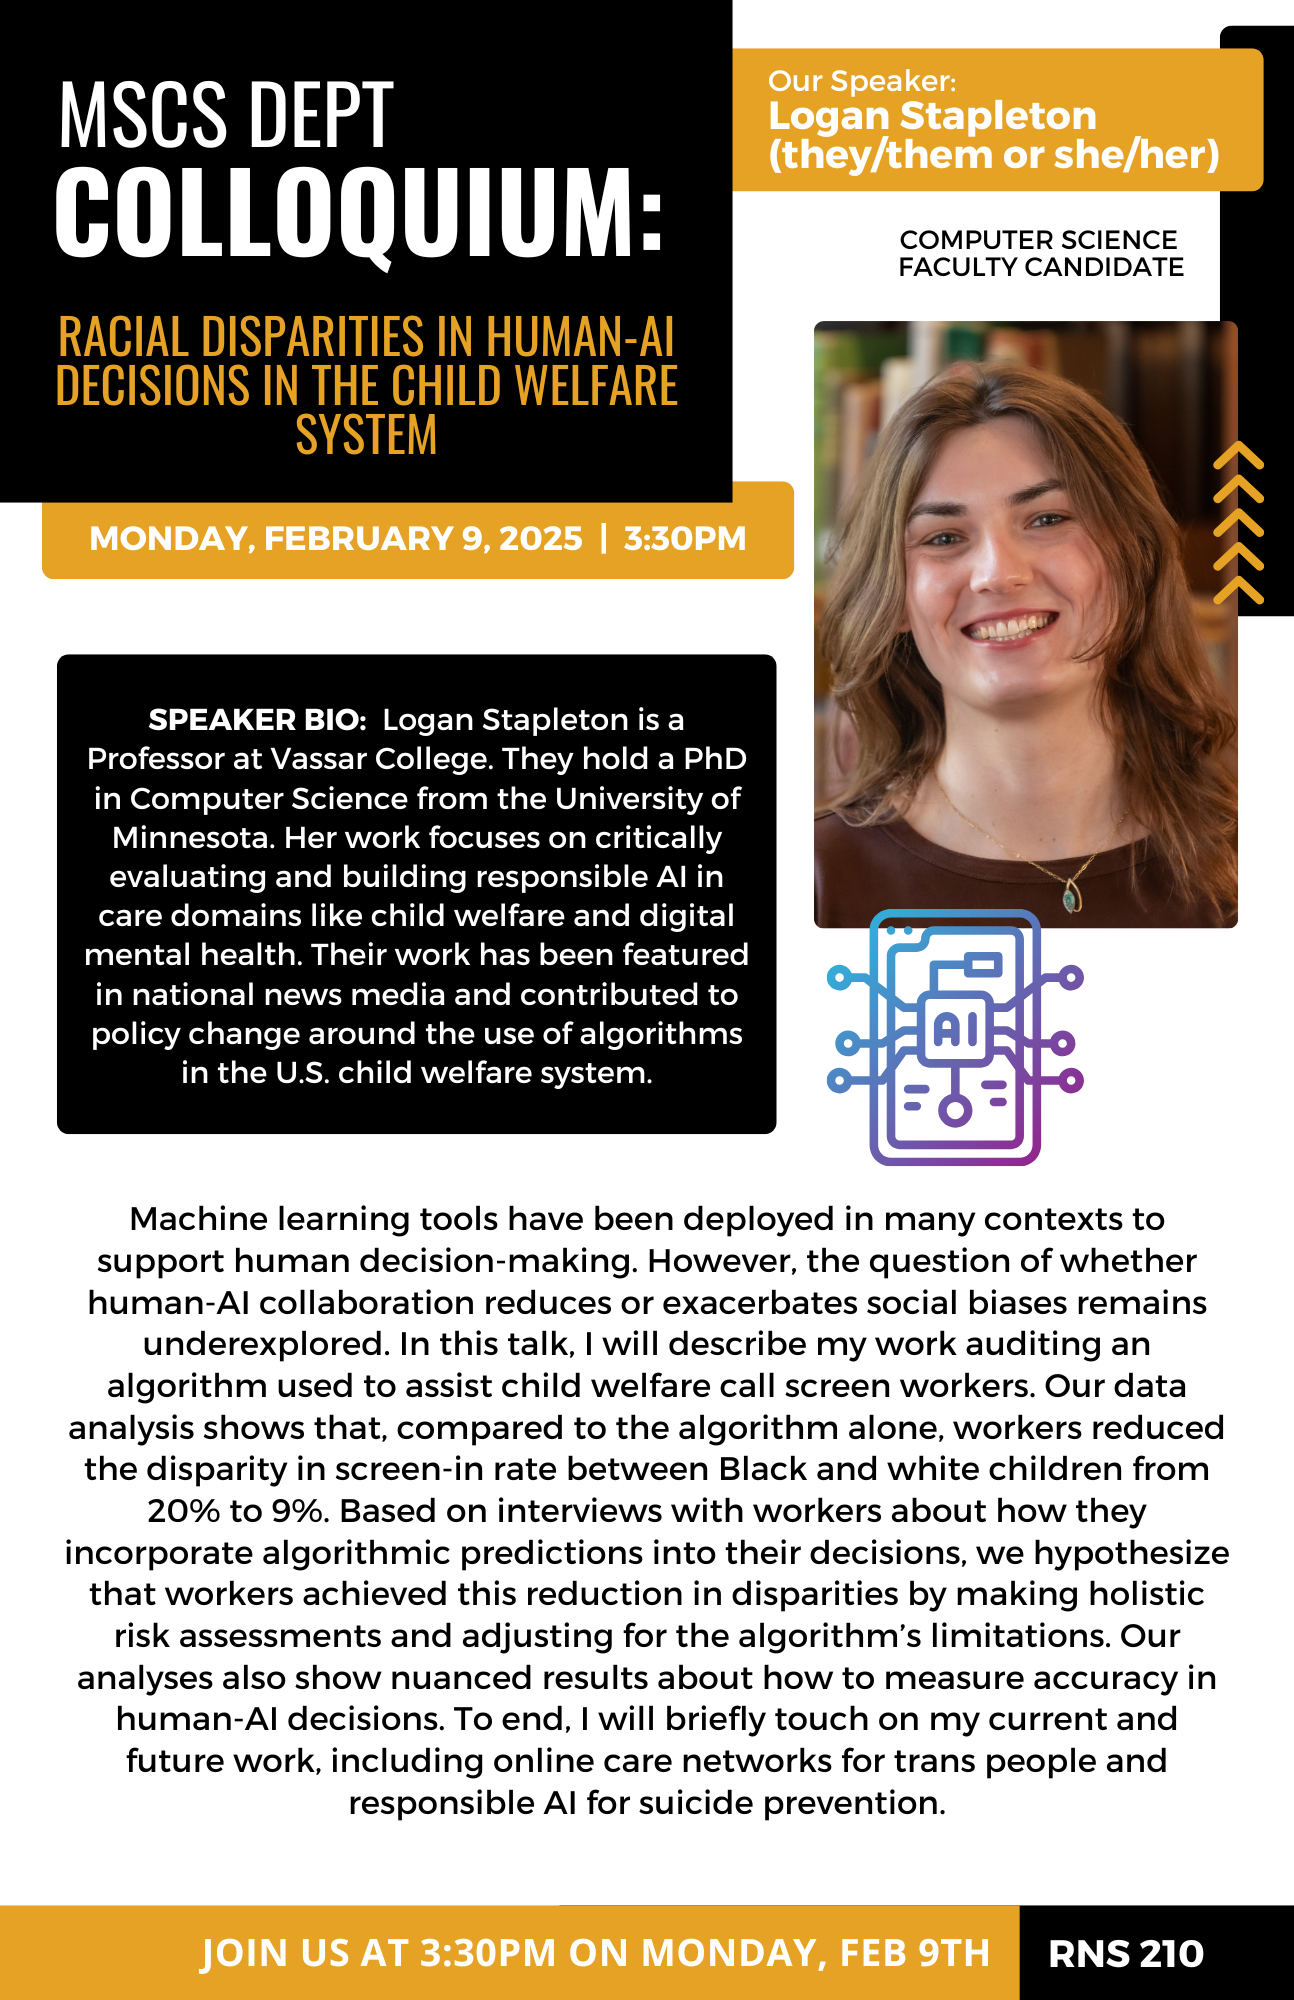
\includegraphics[height=0.9\textheight]{images/Colloquium Logan Stapleton.png}
\end{center}

\begin{center}
    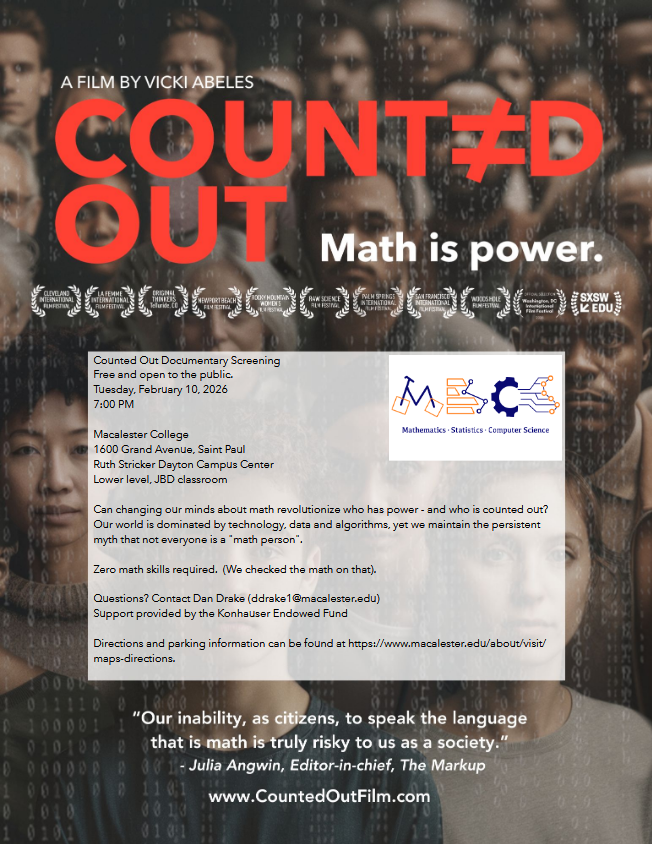
\includegraphics[height=0.9\textheight]{images/Counted Out Flyer.png}
\end{center}

\begin{center}
    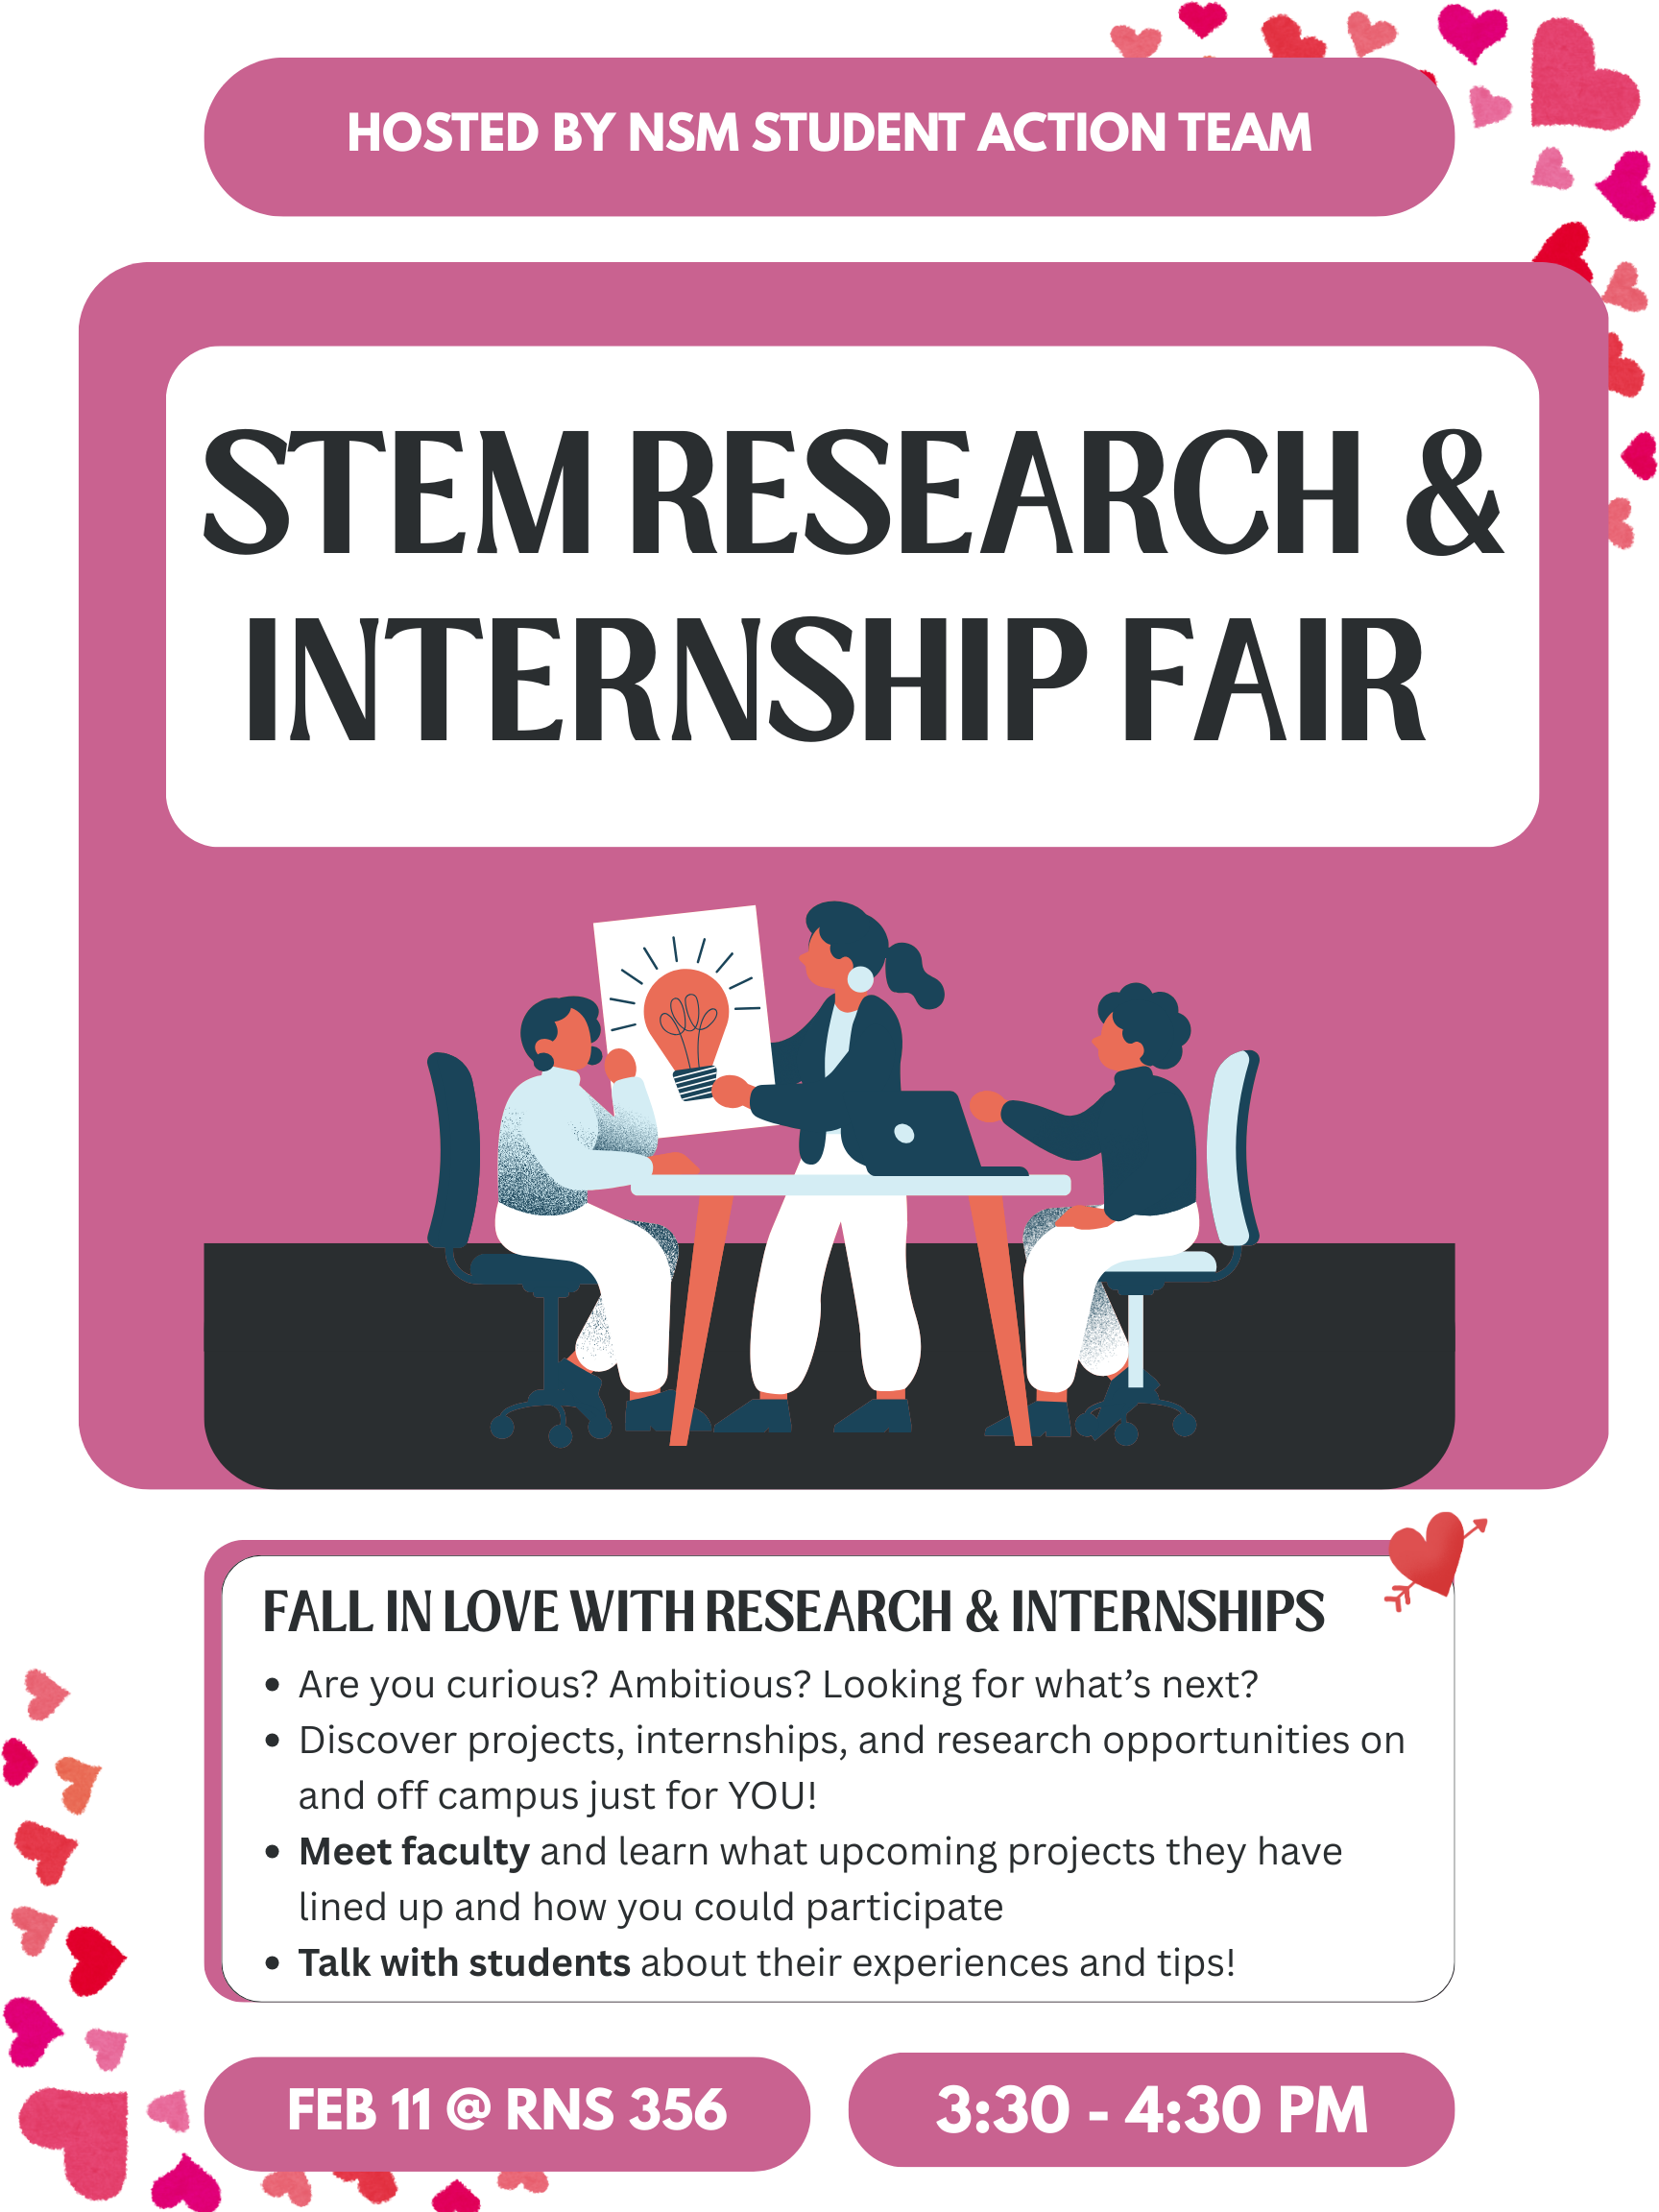
\includegraphics[height=0.9\textheight]{images/Research and Internship Fair Poster 26.png}
\end{center}

\begin{center}
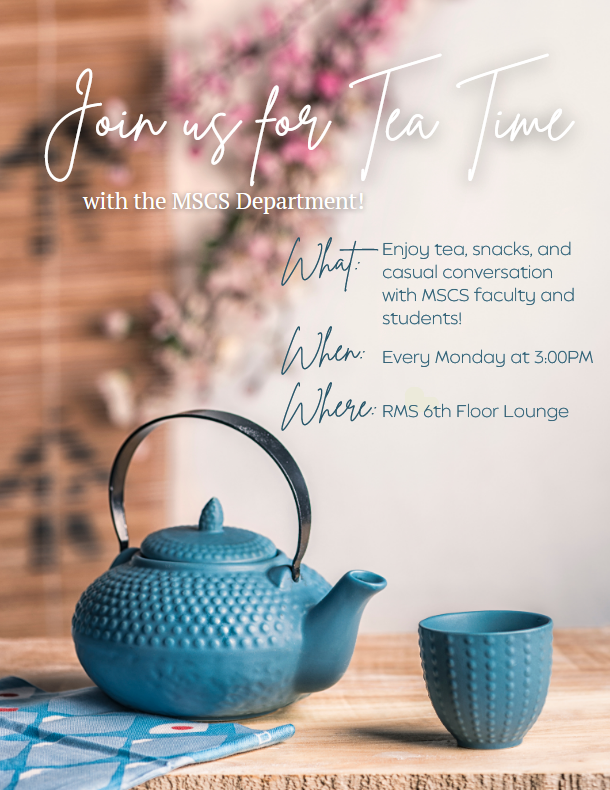
\includegraphics[width=0.9\textwidth]{images/Tea Time Poster.png}
\end{center}

\noindent{To submit an article, event, or anything else for publication in the Mess, email messeditor@stolaf.edu. Visit \href{https://wp.stolaf.edu/mscs/mscs-mess/}{http://wp.stolaf.edu/mscs/mscs-mess/} for a digital archive of previous MSCS Mess issues.}\\
	
\hfill Zach Martin \& Nima Dahir, Editors
	
\hfill Kyle Salois, Faculty Advisor


 

\end{document}